\documentclass[8pt]{beamer}
\usepackage[T2A]{fontenc}                
\usepackage[utf8]{inputenc}  
\usepackage[english, russian]{babel}
\usepackage{indentfirst}
\usepackage{graphicx}

\usetheme{Ilmenau} 
\usefonttheme{structureitalicserif}
\usecolortheme{albatross}


\title{Практикум на ЭВМ.\\ Отчет по четвертому заданию.}
\author{Марков Игорь, Карабутов Дмитрий\\ 312 группа}
\institute{МГУ имени М.В. Ломоносова\\ Москва, Россия}
\date{2018}
 
\begin{document}
 
\frame{\titlepage}
 
 
 
 
\begin{frame}
\frametitle{\centerline{Постановка задачи}}
Для ведения войны с Семью Королевствами требуется оружие, для изготовления которого нужна сталь. Основными поставщиками стали являются две компании : {Westeros Inc.} и {Harpy \& Co}. На данный момент, товар закупается у обеих компаний, но каждая из них предлагает достаточно большую скидку, если контракт на поставку сырья будет заключен эксклюзивно с ней.\\

\bigskip

В связи с этим, поставлена задача проанализировать известные нам данные, из которых требуется сделать соответствующие выводы о качестве стали обоих поставщиков, и решить, с каким из них было бы выгоднее заключить эксклюзивный контракт на закупку стали.\\
\end{frame}
 
 
 
 
\begin{frame}
\frametitle
{Цель работы}
Используя данные о производстве оружия, необходимо провести разведывательный анализ данных с целью ответа на вопрос: "С каким из поставщиков стали следует заключить договор?"
\end{frame}





\begin{frame}

\frametitle{Анализ:\\{\smallКоличество произведенного оружия за каждый месяц}}
\begin{figure}[h]
		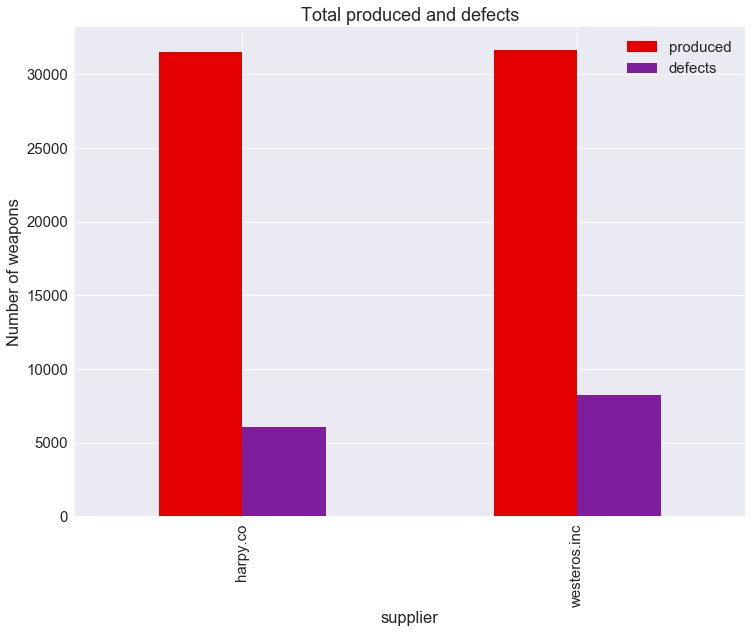
\includegraphics[width=60mm]{1.png}
		\caption{1}
		\label{First}
\end{figure}
По данному графику видно, что, хоть кампания westeros.inc выпускает в среднем оружия больше, чем кампания harpy\&co, в целом разница все же незначительна.\\
\end{frame}





\begin{frame}
\frametitle{Анализ:\\{\small Количество сломанных мечей за все время}}
\begin{figure}[h]
		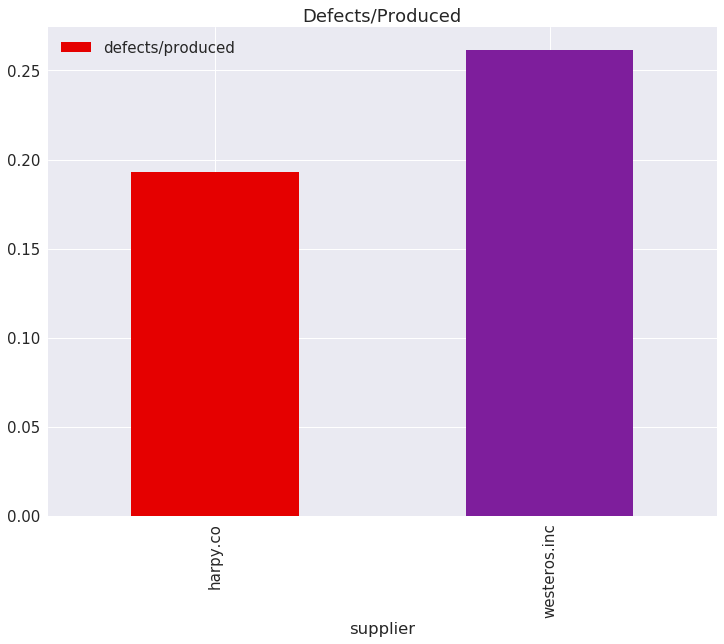
\includegraphics[width=70mm]{2.png}
		\caption{2}
		\label{Second}
\end{figure}
Из графика четко видно, что у кампании harpy\&co сломанных мечей значительно меньше, что является неоспоримым плюсом.
\end{frame}

\begin{frame}
\frametitle{Анализ:\\ {\small Время жизни сломанных мечей}}
\begin{figure}[h]
		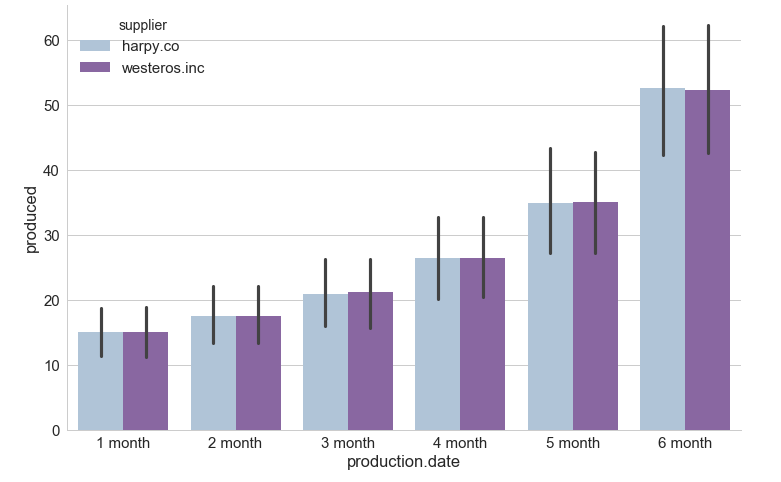
\includegraphics[width=60mm]{3.png}
		\caption{3}
		\label{Third}
\end{figure}
Мы видим, что мечи от Westeros Inc ломаются в целом в первое время использования, наибольшее же количество мечей от Harpy \& Co начинают ломаться, начиная с 4го месяца.
\end{frame}





\begin{frame}

Те же данные, только в процентах:
\begin{figure}[h]
		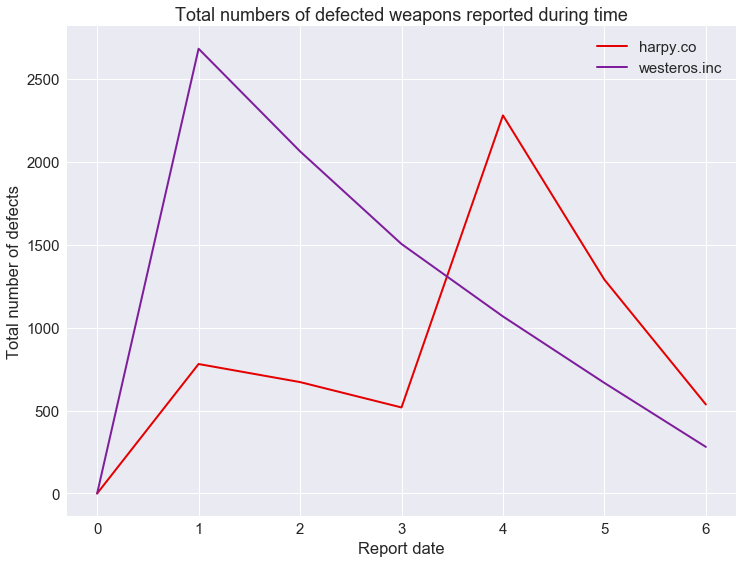
\includegraphics[width=60mm]{4.png}
		\caption{4}
		\label{Fourth}
\end{figure}
\end{frame}




\begin{frame}
\frametitle{Анализ:\\{\smallКоличество мечей, в среднем ломающихся за месяц}}
\begin{figure}[h]
		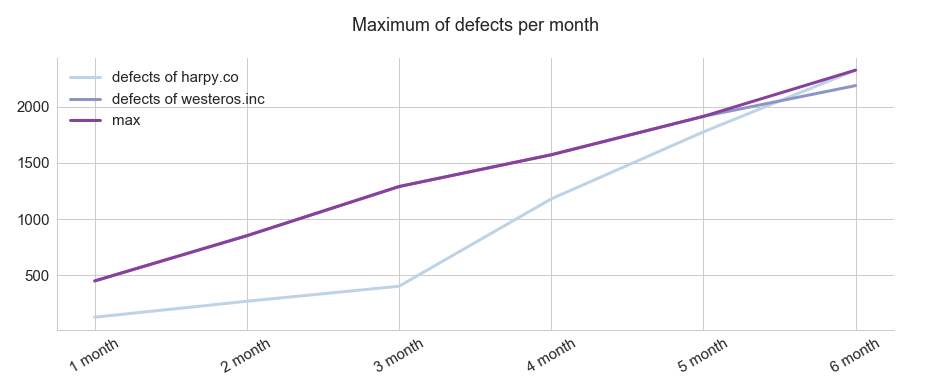
\includegraphics[width=70mm]{5.png}
		\caption{5}
		\label{Fifth}
\end{figure}
На этом графике видно: у кампании harpy \& co в месяц в среднем ломается значительно меньше мечей.\\
\end{frame}



%%%%%%%%%%%%%%%%%%%%%%%
%%%%%вывод вот сюда 
%%%%%%%%%%%%%%%%%%%%%%%
\begin{frame}
\frametitle{Выводы}
Анализируя данные, мы выделели три основных факта:\\
1) Обе кампании производят каждый месяц приблизительно одинаковое количество мечей.\\
2) В среднем у Harpy \& Сo в месяц ломается меньше мечей.\\ 
3) Количество сломанных мечей у Harpy \& Сo более равномерно распределенно по времени.
\\

\bigskip

Исходя из всего вышеперечисленного, мы видим, что Harpy \& Сo - это именно та кампания, с которой нужно заключить контракт в этой долгосрочной войне. 

\end{frame}

\end{document}